%%%%%%%%%%%%%%%%%%%%%%%%%%%%%%%%%%%%%%%%%%%%%%%%%%%%%%%
%                File: OpEx_temp.tex                  %
%                Date: April 30, 2014                 %
%                                                     %
%           LaTeX template file for use with          %
%           OSA's journal Optics Express              %
%                                                     %
%  send comments to Theresa Miller, tmiller@osa.org   %
%                                                     %
% This file requires style file, opex3.sty, under     %
%              the LaTeX article class                %
%                                                     %
%   \documentclass[10pt,letterpaper]{article}         %
%   \usepackage{opex3}                                %
%                                                     %
%                                                     %
%       (c) 2014 Optical Society of America           %
%%%%%%%%%%%%%%%%%%%%%%%%%%%%%%%%%%%%%%%%%%%%%%%%%%%%%%%

%%%%%%%%%%%%%%%%%%%%%%% preamble %%%%%%%%%%%%%%%%%%%%%%%%%%%
\documentclass[10pt,letterpaper]{article}
\usepackage{opex3}
\usepackage{color}

%%%%%%%%%%%%%%%%%%%%%%% begin %%%%%%%%%%%%%%%%%%%%%%%%%%%%%%
\begin{document}

\title{Working Ti}
\author{Author 1$^1$ and Author 2$^{2,*}$}

\address{$^1$Department of Physics and Astronomy, University of Pennsylvania, Philadelphia, PA 19104, USA\\
$^2$Publications Department, Optical Society of America, Washington, D.C., 20036, USA}

\email{$^*$hban@physics.upenn.edu} %% email address is required

% \homepage{http:...} %% author's URL, if desired

%%%%%%%%%%%%%%%%%%% abstract and OCIS codes %%%%%%%%%%%%%%%%
%% [use \begin{abstract*}...\end{abstract*} if exempt from copyright]

\begin{abstract}
Detailed instructions and formatting guidelines for preparing \textit{Optics Express}, \textit{Biomedical Optics Express}, and \textit{Optical Materials Express} manuscripts in \LaTeX. For a simple outline and template, open the simple template file \texttt{OpEx\_temp.txt}. The Express journal simple and extended templates are also available on \url{http://www.writelatex.com}. OSA encourages the use of this free online collaborative tool for writing your OSA article.
\end{abstract}

\ocis{(000.0000) General.} % REPLACE WITH CORRECT OCIS CODES FOR YOUR ARTICLE, MINIMUM OF TWO; Avoid using the OCIS codes for “General” or “General science” whenever possible.
%For a complete list of OCIS codes, visit: http://www.opticsinfobase.org/submit/ocis/

%%%%%%%%%%%%%%%%%%%%%%% References %%%%%%%%%%%%%%%%%%%%%%%%%
\begin{thebibliography}{99}
\bibitem{bib1}P. J. Harshman, T. K. Gustafson, and P. Kelley, "Title of paper," J. Chem. Phys. {\bf 3}, (to be published).

\bibitem{gallo99} K. Gallo and G. Assanto, ``All-optical diode based on second-harmonic generation in an asymmetric waveguide,'' \josab {\bf 16}(2), 267--269 (1999).

\bibitem{Masters98a} B. R. Masters, ``Three-dimensional microscopic tomographic imagings of the cataract in a human lens in vivo,'' \opex {\bf 3}(9), 332--338 (1998).

\bibitem{Oron03} D. Yelin,  D. Oron,  S. Thiberge,  E. Moses, and Y. Silberberg, ``Multiphoton plasmon-resonance microscopy,'' \opex {\bf 11}(12), 1385--1391 (2003).

\bibitem{samplefig}
B.~N.~Behnken, G.~Karunasiri, D.~R.~Chamberlin, P.~R.~Robrish, and J.~Faist,
``Real-time imaging using a 2.8~THz quantum cascade laser and uncooled infrared microbolometer camera,''
\ol \textbf{33}(5), 440--442 (2008).

\end{thebibliography}

%%%%%%%%%%%%%%%%%%%%%%%%%%  body  %%%%%%%%%%%%%%%%%%%%%%%%%%
\section{Introduction}
Adherence to the specifications listed in this template is essential for efficient review and publication of submissions. Since OSA does not routinely perform copyediting and typesetting for this journal, use of the template is critical to providing a consistent appearance. Proper reference format is especially important (see Section \ref{sec:refs}).

\section{\texttt{opex3.sty} and required \LaTeX{} packages}
Page layout is set with the \texttt{geometry} package for US Letter paper. \texttt{opex3.sty} uses the following package files:

\begin{itemize}
\item \texttt{geometry} \ (page layout)
\item \texttt{color, graphicx} \ (replaces \texttt{graphics}; has preset options)
\item \texttt{mathptmx, courier, helvet} \ (Times, Courier, and Helvetica fonts)
\end{itemize}

The latest versions of these standard package files can be obtained at CTAN: the Comprehensive TeX Archive Network, \url{http://www.ctan.org}.

The command \verb+\usepackage{ae}+ can be invoked to revert font to Computer Modern, although we prefer to publish with Times (with \texttt{mathptmx.sty}) for consistency.

\section{Multiple corresponding authors}

There are two options for indicating multiple corresponding authorship, and they are formatted quite differently. The first format would be as follows, still using the asterisk to denote one of the authors:

\begin{verbatim}
\author{Dan McDonald$^{1,3}$ and Theresa Miller$^{2,*}$}

\address{$^{1}$Peer Review, Publications Department,
Optical Society of America,\\ 2010 Massachusetts Avenue NW,
Washington, D.C., 20036, USA\\
$^{2}$Publications Department, Optical Society of America,\\
2010 Massachusetts Avenue NW, Washington, D.C., 20036, USA\\
$^{3}$dmcdonold@osa.org}

\email{*opex@osa.org}
\end{verbatim}

This format will generate the following appearance:

\author{Dan McDonald$^{1,3}$ and Theresa Miller$^{2,*}$}

\address{$^{1}$Peer Review, Publications Department, Optical Society of America,\\ 2010 Massachusetts Avenue NW, Washington, D.C., 20036, USA\\
$^{2}$Publications Department, Optical Society of America,\\ 2010 Massachusetts Avenue NW, Washington, D.C., 20036, USA\\
$^{3}$dmcdonold@osa.org}

\email{*opex@osa.org}

The second format forgoes the asterisk and sets all email addresses equally within the affiliations. Please note that this format does not use the \verb+\email{}+ field at all.
\begin{verbatim}
\author{Dan McDonald$^{1,3}$ and Theresa Miller$^{2,4}$}

\address{$^{1}$Peer Review, Publications Department,
Optical Society of America,\\ 2010 Massachusetts Avenue NW,
Washington, D.C., 20036, USA\\
$^{2}$Publications Department, Optical Society
of America,\\ 2010 Massachusetts Avenue NW,
Washington, D.C., 20036, USA\\
$^{3}$dmcdonold@osa.org\\
$^{4}$opex.osa.org}
\end{verbatim}

This format will generate the following appearance:

\author{Dan McDonald$^{1,3}$ and Theresa Miller$^{2,4}$}

\address{$^{1}$Peer Review, Publications Department, Optical Society of America,\\ 2010 Massachusetts Avenue NW, Washington, D.C., 20036, USA\\
$^{2}$Publications Department, Optical Society of America,\\ 2010 Massachusetts Avenue NW, Washington, D.C., 20036, USA\\
$^{3}$dmcdonold@osa.org\\
$^{4}$opex.osa.org}

These are the preferred express journal formats for multiple corresponding authorship, and either may be used.

\section{Abstract}
The abstract should be limited to approximately 100 words. It should be an explicit summary of the paper that states the problem, the methods used, and the major results and conclusions. It also should contain the relevant key words that would allow it to be found in a cursory computerized search. If the work of another author is cited in the abstract, that citation should be written out without a number, [e.g., author, journal, volume, first page, and year (T. Miller, Opt. Express {\bf 22}, 1234 (2014).)], and a separate citation should be included in the body of the text. The first reference cited in the main text must be [1]. Do not include numbers, bullets, or lists inside the abstract.

\section{Figures, tables, and multimedia}

\subsection{Figures and tables}

OSA express journals encourage authors to submit color and multimedia figures with their manuscripts. Figures and tables should be placed in the body of the manuscript.

\begin{figure}[h]
\centering\includegraphics[width=7cm]{opexfig1}
\caption{Sample caption (Ref. \cite{Oron03}, Fig. 2).}
\end{figure}

\noindent Standard \LaTeX{} environments should be used to place tables and figures:
\begin{verbatim}
\begin{figure}[htbp]
\centering\includegraphics[width=7cm]{opexfig1}
\caption{Sample caption (Ref. \cite{Oron03}, Fig. 2).}
\end{figure}
\end{verbatim}

\subsection{Multimedia and supplementary materials in OSA journals}

Most OSA journals allow authors to include supplementary materials as integral parts of a manuscript. Such materials are subject to the same editorial standards and peer-review procedures as the rest of the manuscript. Authors who wish to submit supplementary materials must adhere to the following guidelines. Note that, with the exception of \textit{Optica}, OSA journals require supplementary material consisting of additional text, figures, tables, equations, etc., to be included as an appendix to the manuscript and not as separate supplementary files.

To ensure consistent presentation, broad accessibility, and long-term archiving for multimedia files, please follow these guidelines on presentation. Please note that to create text color for media links, use of the color.sty package and the command \verb|\textcolor{blue}{Media}| is preferred to using the command \verb|\url{Media}|.

\begin{figure}[h]
\centering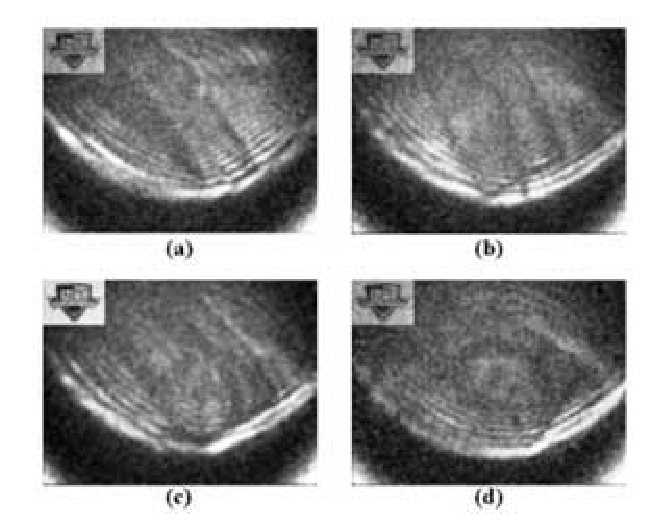
\includegraphics{opexfig2}
\caption{Single-frame excerpts from video recordings of metallic objects concealed by opaque plastic tape. (a) Utility blade (\textcolor{blue}{Media~1}). (b) Dentist's pick (\textcolor{blue}{Media~2}). (c) Paper clip (\textcolor{blue}{Media~3}). (d) Plastic/wire tie twisted into the shape of a loop (\textcolor{blue}{Media~4}). (Sample figure adapted from \cite{samplefig}.)}
\end{figure}

\begin{verbatim}
\begin{figure}[h]
\centering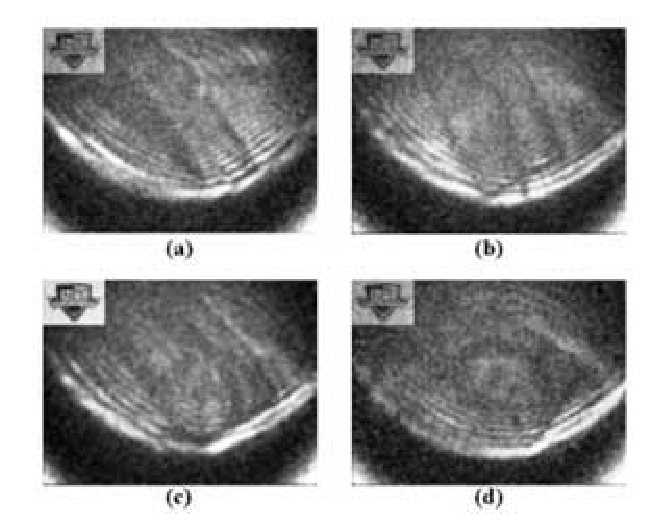
\includegraphics{opexfig2}
\caption{Single-frame excerpts from video recordings of metallic
objects concealed by opaque plastic tape. (a) Utility
blade (\textcolor{blue}{Media~1}). (b) Dentist's
pick (\textcolor{blue}{Media~2}). (c) Paper
clip (\textcolor{blue}{Media~3}).
(d) Plastic/wire tie twisted into the shape of a
loop (\textcolor{blue}{Media~4}). (Sample figure adapted
from \cite{samplefig}.)}
\end{figure}
\end{verbatim}

Acceptable file types are MOV, AVI, MPG, and MP4. There are a variety of software applications to aid in creating this file format. OSA accepts the following QuickTime compressor types: Video, Graphics, Animation, Motion JPEG, Cinepak, and Uncompressed/None. OSA does not accept the Indeo 5 compressor.

The following multimedia guidelines will help with the submission process:
\begin{itemize}
\item 15 MB is the recommended maximum multimedia file size.
\item Use one of the accepted compression codecs to minimize file sizes.
\item 720 x 480 pixels (width by height) is the recommended screen size.
\item Insert a representative frame from each movie in the manuscript as a figure.
\item Videos must be playable using the free version of QuickTime on the Mac and PC.
\item Animations must be formatted into a standard video file.
\end{itemize}
Please refer to the online style guide \\ (\mbox{\url{http://www.opticsinfobase.org/oe/submit/style/multimedia.cfm}}) for more detailed instructions on acceptable multimedia formats for audio and tabular data.


\section{Mathematical and scientific notation}

\subsection{Displayed equations} Displayed equations should be centered.
Equation numbers should appear at the right-hand margin, in
parentheses:
\begin{equation}
H = \frac{1}{2m}(p_x^2 + p_y^2) + \frac{1}{2} M{\Omega}^2
     (x^2 + y^2) + \omega (x p_y - y p_x).
\end{equation}

All equations should be numbered in the order in which they appear
and should be referenced  from within the main text as Eq. (1),
Eq. (2), and so on [or as inequality (1), etc., as appropriate].

\subsection{Inline math} To help with conversion, place all math in a proper math environment. For example, expression \mbox{$3\times 4 = 12$} should be set this way, \texttt{\$3$\backslash$times 4=12\$}, not this way, \texttt{3 \$$\backslash$times\$4=12}. Simple fractions for inline math
should use parentheses when necessary to avoid ambiguity, for
example, to distinguish between $1/(n-1)$ and $1/n-1$.  Exceptions
to this are the proper fractions such as $\frac{1}{2}$, which are
better left in this form. Summations and integrals that appear
within text such as $\frac{1}{2}{\sum }_{n=1}^{n=\infty} (n^2 -
2n)^{-1}$ should have limits placed to the right of the symbol to
reduce white space.

\subsection{General guidelines on notation} Notation must be
legible, clear, compact, and consistent with standard usage. In
general, acronyms should be defined at first use. Adherence to the
following guidelines will greatly assist the production process:

\paragraph*{\bf Radical signs.}
When possible, avoid oversized radical signs
by using the notation of a superscript $1/2$. For example, change
$\sqrt{(a + b)(a - c)}$ to $[(a + b)(a - c)]^{1/2}$.

\paragraph*{\bf Exponentials.} Avoid tiny superscripts of exponential $e$ (e.g.,
$e^{jkl})$ by using the alternative \verb+\exp+ notation,
$\exp(jkl)$.

\paragraph*{\bf Variables and vectors.}
Set single-letter variables in italics $(k)$. Set three-vectors in
boldface $(\mathbf{k})$. Functions, derivative ``d,''
abbreviations, and multiletter identifiers should be set in roman
(plain) type  ($\alpha \cos, \int\!\dots{\rm d}x, k^{\rm out}$).

\paragraph*{\bf Multiplication.}
In general, close up multiplied terms $(p_yp_x)$;
use $\times$ if multiplication sign is essential $(2 \times
10^{-2})$ or for continuation in displayed equations. Use raised dot only for scalar product $(\mathbf{k \cdot k})$.

\paragraph*{\bf Fences.}
For simple bracketing the usual order of parentheses and brackets
is $\{ \, [  \, (  \,  \{  \, [  \, (  \, |  \, )  \, ]  \, \} \,
)  \, ]  \, \}$.


\paragraph*{\bf Metric system.}
The metric system is used in OSA journals. If nonmetric units are
essential (e.g., for parts specifications), conversion should be
given at first mention:  ``. . . a $\frac{1}{4}$\,-in. bolt \mbox{(1 in.
= 2.54 cm).''}

\subsection{Acknowledgments} Acknowledgments, if included, should
appear at the end of the document, just before the references. The
number of a grant or contract should be omitted unless its
inclusion is required by the agency supporting the research. Use
the command \verb+\section*{Acknowledgments}+  to create a
nonnumbered section heading.

\section{References}
\label{sec:refs}
Proper formatting of references is extremely important, not only for consistent appearance but also for accurate electronic tagging. Please follow the guidelines provided below on formatting, callouts, and use of Bib\TeX.

\subsection{Formatting reference items}
Each source must have its own reference number. Footnotes (notes at the bottom of text pages) are not used in OSA journals. References require all author names, full titles, and inclusive pagination. Here are some examples of how to set the most common reference types:

\begin{description}
\item[Journal paper] \hfill\\
{\it Do not include web addresses in journal citations.}

C. van Trigt, ``Visual system-response functions and estimating reflectance,'' %\josaa
   J. Opt. Soc. Am. A {\bf 14}(4), 741--755 (1997).

S. Yerolatsitis, I. Gris-S\'anchez, and T. A. Birks,
``Adiabatically-tapered fiber mode multiplexers,'' Opt. Express {\bf 22}(1), 608--617 (2014).

\item[Journal paper identified by paper number] \hfill\\
{\it The paper number is sufficient. There is no need to give the number of pages.}

L. Rippe, B. Julsgaard, A. Walther, Y. Ying, and S. Kr\"oll,
``Experimental quantum-state tomography of a solid-state qubit,'' Phys. Rev. A {\bf 77}, 022307 (2008).

\item[Book] \hfill\\
T. Masters, {\it Practical Neural Network Recipes in C++} (Academic, 1993).

F. Ladouceur and J. D. Love, \textit{Silica-Based Buried Channel Waveguides and Devices} (Chapman \& Hall, 1995), Chap. 8.

\item[Article in a book] \hfill\\
D. F. Edwards, ``Silicon (Si),'' in {\it Handbook of Optical Constants of Solids,} E. D. Palik, ed. (Academic, 1985).

\item[Paper in a published conference proceedings] \hfill\\
R. E. Kalman, ``Algebraic aspects of the generalized inverse of a
rectangular matrix,'' in {\it Proceedings of Advanced Seminar on
Generalized Inverse and Applications,} M. Z. Nashed, ed. (Academic, 1976), pp. 111--124.

\item[Paper published in an OSA conference proceedings] \hfill\\
R. Craig and B. Gignac, ``High-power 980-nm pump lasers,'' in
{\it Optical Fiber Communication Conference}, Vol. 2 of 1996 OSA Technical Digest Series
(Optical Society of America, 1996), paper ThG1.

\item[Paper presented at a meeting/from an unpublished conference proceeding] \hfill\\
D. Steup and J. Weinzierl, ``Resonant THz-meshes,'' presented at the
Fourth International Workshop on THz Electronics,
Erlangen-Tennenlohe, Germany, 5--6 Sept. 1996.

\item[SPIE proceedings] \hfill\\
S. K. Griebel, M. Richardson, K. E. Devenport, and H. S. Hinton,
``Experimental performance of an ATM-based buffered hyperplane
CMOS-SEED smart pixel array,'' Proc. SPIE {\bf 3005}, 254--256 (1997).

{\it For later SPIE proceedings with a paper number, cite just the number and not any page information.}

S. Gu, F. Shao, G. Jiang, F. Li, and M. Yu,
``An objective visibility threshold measurement method for asymmetric stereoscopic images,''
Proc. SPIE {\bf 8205}, 820505 (2011).

\item[IEEE proceedings] \hfill\\
T. Darrel and K. Wohn, ``Pyramid based depth from focus,'' in
{\it Proceedings of IEEE Conference on Computer Vision and Pattern
Recognition} (IEEE, 1988), pp. 504--509.

\item[Paper accepted for publication] \hfill\\
D. Piao, ``Cancelation of coherent artifacts in optical coherence tomography imaging,'' Appl. Opt. (to be published).

D. W. Diehl and T. D. Visser,
"Phase singularities of the longitudinal field components in the focal region of a high-aperture optical system,"
J. Opt. Soc. Am. A, doc. ID 56789 (posted 11 November 2005, in press).

\item[Manuscript in preparation] \hfill\\
J. Q. Smith, Laboratory for Laser Energetics, University of Rochester, 250 East River Road, Rochester, New York 14623, USA, and K. Marshall are preparing a manuscript to be called ``Optical aspects in liquid crystals.''

\item[Personal communication] \hfill\\
T. Miller, Publications Department, Optical Society of
America, 2010 Massa\-chusetts Avenue, N.W., Washington, D.C.,
20036 (personal communication, 2010).

\item[Internet links] \hfill\\
Extreme Networks white paper, ``Virtual metropolitan area networks,'' (Extreme Networks, 2001), \texttt{http://www.extremenetworks.com/technology/
whitepapers/vMAN.asp}.

A. G. Ramm, ``Invisible obstacles,'' \texttt{http://www.arxiv.org/abs/math-ph
/0608034}.

\end{description}

The commands \verb+\begin{thebibliography}{}+ and \verb+\end{thebibliography}+ format the section according to standard style, showing the title {\bf References and links}.  Use the \verb+\bibitem{label}+ command to start each reference.

\subsection{Formatting reference citations}
References should be numbered consecutively in the order in which they are referenced in the body of the paper. Set reference callouts with standard \verb+\cite{}+ command or set manually inside square brackets [1].

To reference multiple articles at once, simply use the cite command with a comma separating the reference labels, e.g. \verb+\cite{gallo99,Masters98a,Oron03}+, produces \cite{gallo99,Masters98a,Oron03}. Using the \texttt{cite.sty} package will make these citations appear like so: [2--4].

\subsection{Bib\TeX}
\label{sec:bibtex}
Bib\TeX{} may be used to create a file containing the references, whose contents (i.e., contents of \texttt{.bbl} file) can then be pasted into the bibliography section of the \texttt{.tex} file. A new Bib\TeX{} style file, \texttt{osajnl.bst}, is provided.

To assist authors with journal abbreviations in references, standard abbreviations for 31 commonly cited journals have been included as macros within opex3.sty.  The abbreviations are shown in Table 1.

\begin{table}[htbp]
\centering\caption{Standard abbreviations
 for commonly cited journals.}
\begin{tabular}{lp{1.7in}|lp{1.7in}}
\hline
Macro        & Abbreviation                & Macro        & Abbreviation          \\ \hline
\verb+\ao+   & Appl.\  Opt.\               &   &       \\
\verb+\aop+  & Adv. Opt. Photon.           & \verb+\jpp+  & J. Phys.              \\
\verb+\ap+   & Appl.\  Phys.\              & \verb+\nat+  & Nature                \\
\verb+\apl+  & Appl.\ Phys.\ Lett.\        & \verb+\oc+   & Opt.\ Commun.\        \\
\verb+\apj+  & Astrophys.\ J.\             & \verb+\opex+ & Opt.\ Express         \\
\verb+\as+   & Appl. Spectrosc.            & \verb+\ol+   & Opt.\ Lett.\          \\
\verb+\bell+ & Bell Syst.\ Tech.\ J.\      & \verb+\ome+  & Opt.\ Mater.\ Express \\
\verb+\boe+  & Biomed.\ Opt.\ Express      & \verb+\opn+  & Opt.\ Photon.\ News   \\
\verb+\jqe+ & IEEE J.\ Quantum Electron.\  & \verb+\pl+   & Phys.\ Lett.\         \\
\verb+\assp+ & IEEE Trans.\ Acoust.\ Speech Signal Process.\ & \verb+\pr+ & Photon.\ Res.\ \\
\verb+\aprop+ & IEEE Trans.\  Antennas Propag.\    & \verb+\prb+ & Phys.\ Rev.\ A   \\
\verb+\mtt+ & IEEE Trans.\ Microwave Theory Tech.\ & \verb+\prc+ & Phys.\ Rev.\ B   \\
\verb+\iovs+ & Invest.\ Ophthalmol.\ Vis.\ Sci.\   & \verb+\prd+ & Phys.\ Rev.\ C   \\
\verb+\jcp+ & J.\ Chem.\ Phys.\            & \verb+\pre+ & Phys.\ Rev.\ D   \\
\verb+\jmo+ & J.\ Mod.\ Opt.\              & \verb+\pra+ & Phys.\ Rev.\ E   \\
\verb+\jocn+ & J.\ Opt.\ Commun.\ Netw.\   & \verb+\prl+ & Phys.\ Rev.\ Lett.\    \\
\verb+\jon+ & J.\ Opt.\ Netw.\             & \verb+\rmp+ & Rev.\ Mod.\ Phys.\    \\
\verb+\josa+ & J.\ Opt.\ Soc.\ Am.\        & \verb+\pspie+ & Proc.\ Soc.\ Photo-Opt.\ Instrum.\ Eng.\   \\
\verb+\josaa+ & J.\ Opt.\ Soc.\ Am.\ A     & \verb+\sjqe+ & Sov.\ J.\ Quantum Electron.\   \\
\verb+\josab+ & J.\ Opt.\ Soc.\ Am.\ B     & \verb+\vr+ & Vision Res.\   \\ \hline
\end{tabular}
\end{table}


\section{Conclusion}
After proofreading the manuscript, compress your .TEX manuscript file and all figures (which should be in EPS format, or PDF format if you are using PDF-\LaTeX) in a ZIP, TAR or TAR-GZIP package. Prism, OSA’s article tracking system, will process in \LaTeX mode by default but will use PDF-\LaTeX if PDF figure files are detected. Note: TAR or TAR-GZIP is no longer required. All files must be referenced at the root level (e.g., file \texttt{figure-1.eps}, not \texttt{/myfigs/figure-1.eps}). If there is video or other multimedia, the associated files should be uploaded separately.

\end{document}
